\documentclass[12pt]{article}
\oddsidemargin=0.0in
\evensidemargin=0.0in
\textwidth=6.5in
\topmargin=-0.65in
\textheight=9.5in
\usepackage{hyperref}
\usepackage{amsmath}
\usepackage{wasysym}
\usepackage{graphicx}
 
\begin{document}
\pagestyle{empty}
 
\begin{center}
{\LARGE {\bf Homework Two}}\\
\bigskip
{\Large {\bf Calculus I}}\\
\bigskip
{\Large {\bf College of the Atlantic}}\\
\bigskip
{ {\bf Due Friday, January 20, 2023}}\\ 
\end{center}
\medskip


\noindent There are three parts to this assignment.\\

\noindent {\bf Part 1: WeBWorK}.  Do Homework 02 on WeBWorK. The WeBWorK page is here:
\url{https://webwork-hosting.runestone.academy/webwork2/coa-feldman-es3012m-winter2023}.
I recommend doing the WeBWorK part of the homework first.  This will
enable you to benefit WeBWorK's instant feedback before you do part
two.\\ 


\noindent {\bf Part 2: A Coding Exercise}. Do the following on a new
google colab notebook. When you are done, please attach the notebook
on google classroom. Write a notebook that does the following:
\begin{enumerate}
  \setlength{\itemsep}{-1mm}
\item Use the {\tt def} command to define the function
  \begin{equation}
    f(x) \, = \, 10e^{-0.05x}\cos(10x/\pi) \;.
  \end{equation}
\item Plot the function from $x=0$ to $x=50$.
  \item Make sure your plot looks nice and smooth.
\end{enumerate}

\noindent Hints/reminders:
\begin{itemize}
  \setlength{\itemsep}{-1mm}
\item Remember to import the modules you need.
\item Remember to put {\tt np.} in front of any math functions you
  need from {\tt numpy}.
\item The exponential function is {\tt exp}.  In other words:
  \begin{equation}
    e^{-5t} \, \text{ is {\tt exp(-5*t)} in python.}
  \end{equation}
\item Multiplication is indicated by a {\tt *}.  I.e., it's {\tt
  10*x}, not {\tt 10x}. \\
\end{itemize}


\noindent {\bf Part 3: Non-WeBWorK problems}.  Here are some
instructions for how to submit this part of the assignment.
\begin{itemize}
  \setlength{\itemsep}{-1mm}
\item Do the problems by hand using pencil (or pen) and paper.
  There is no need to type this assignment.
\item If you like working on a tablet, go for it. 
\item Make a pdf scan of your work using genius scan or some
  similar scanning app.  Please make the homework into a single
  pdf, not multiple pdfs.
  \item Please, I am begging you, please don't scan your work in
    sideways. \smiley{}
\item Submit the assignment on google classroom.  Please don't
  email it to me.  %(Between my two classes I will be receiving
  %around 60 assignments a week.  Keeping track of them all in email 
  %is challenging.)
\item If you want, you can do the non-WeBWorK and coding in pairs and
  submit only one assignment for the two of you. \\
\end{itemize}

\noindent Here is a non-WeBWorK problem.\\

\noindent The figure below shows the rate at which sleet is falling,
in units of centimeters per hour, during the first three hours of a
sleet storm in Maine. 


\begin{figure}[h]
\begin{center}
\vspace{1mm}
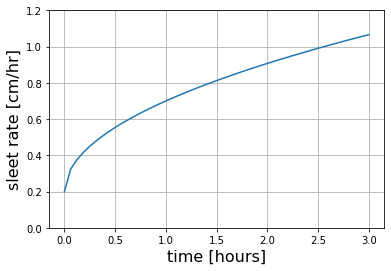
\includegraphics[width=5.0in]{sleet.png}
\vspace{-1mm}
\caption{The rate that sleet is falling, in units of cm/hr, during the
  first three hours of a sleet/ice storm in Maine.}
\vspace{-5mm}
\label{fig:graph1}
\end{center}
\end{figure}
%\vspace{0mm}


\begin{enumerate}
  \item Come up with a lower estimate for the total amount of sleet
    that has fallen during the first three hours of the storm. use
    $\Delta t = 0.5$ hours.
  \item Come up with an upper estimate for the total amount of sleet
    that has fallen during the first three hours of the storm. use
    $\Delta t = 0.5$ hours.
  \item As $\Delta t$ gets smaller and smaller, the upper and lower
    estimates get closer and closer to each other. How small a $\Delta
    t$ wold you need to choose so that the difference between the
    upper and lower estimates was $0.1$ cm.
\end{enumerate}



%\begin{enumerate}
%\setlength{\itemsep}{-1mm}
%  \item Determine an equation for the linear function that generates
%    the values in the table below.  
%
%\begin{center}
%\begin{tabular}{|| l | l ||}
%\hline $x$ & $f(x)$ \\
%\hline
%5.2 & 27.8 \\
%5.3 & 29.2 \\
%5.4 & 30.6 \\
%5.5 & 32.0 \\
%5.6 & 33.4 \\
%\hline
%\end{tabular}
%\end{center}

%\end{enumerate}




\end{document}
